\documentclass[11pt]{article}

\usepackage{fullpage}
\usepackage{graphicx}
\usepackage{amsmath}
\usepackage{amssymb}
\usepackage{amsthm}
\usepackage{fancyvrb}

\parindent0in
\pagestyle{plain}
\thispagestyle{plain}

\newcommand{\myname}{Mehshan Mustafa}
\newcommand{\dated}{\today}

\newenvironment{theorem}[2][Theorem]{\begin{trivlist}
\item[\hskip \labelsep {\bfseries #1}\hskip \labelsep {\bfseries #2.}]}{\end{trivlist}}
\newenvironment{lemma}[2][Lemma]{\begin{trivlist}
\item[\hskip \labelsep {\bfseries #1}\hskip \labelsep {\bfseries #2.}]}{\end{trivlist}}
\newenvironment{exercise}[2][Exercise]{\begin{trivlist}
\item[\hskip \labelsep {\bfseries #1}\hskip \labelsep {\bfseries #2.}]}{\end{trivlist}}
\newenvironment{problem}[2][Problem]{\begin{trivlist}
\item[\hskip \labelsep {\bfseries #1}\hskip \labelsep {\bfseries #2.}]}{\end{trivlist}}
\newenvironment{question}[2][Question]{\begin{trivlist}
\item[\hskip \labelsep {\bfseries #1}\hskip \labelsep {\bfseries #2.}]}{\end{trivlist}}
\newenvironment{corollary}[2][Corollary]{\begin{trivlist}
\item[\hskip \labelsep {\bfseries #1}\hskip \labelsep {\bfseries #2.}]}{\end{trivlist}}
\newenvironment{solution}{\begin{proof}[Solution]}{\end{proof}}
\newenvironment{idea}[2][Proof Idea.]{\textit{#1} #2}

\begin{document}
\textbf{Introduction to the Theory of
Computation}\hfill\textbf{\myname}\\[0.01in]
\textbf{Chapter 1: Reqular Languages}\hfill\textbf{\dated}\\
\smallskip\hrule\bigskip

\begin{problem}{1.31}
Let $C_{n} = \{x \ | \ x \ is \ a \ binary \ number \ that \ is \ a \ multiple \ of\  n \}$. Show that for each $n \geq 1$, the language $C_{n}$ is regular.
\end{problem}

\begin{idea}
Design a finite automaton that simulates long division of $x$ by $n$. Such a finite automaton will have a state for each possible remainder 0 to $n-1$. State 0 will be the only accept state.
\begin{center}
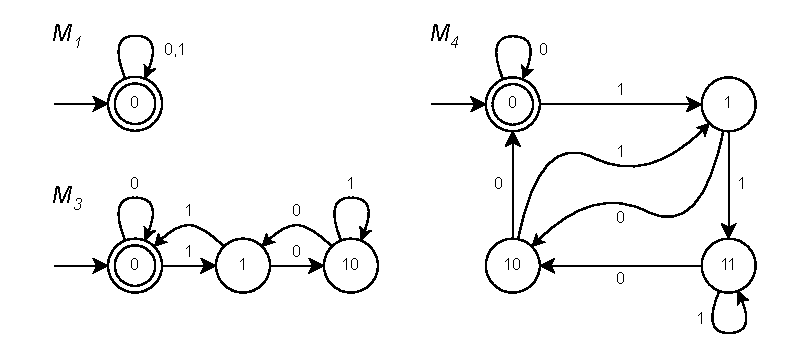
\includegraphics[scale=1.0]{Figures/Problem1.37.pdf} \\
State diagrams of DFAs that recognize $B_{1}$, $B_{3}$ and $B_{4}$. In each DFA, the states are binary numbers corresponding to each possible remainder.
\end{center}
\end{idea}

\begin{proof}
The proof is by construction. Construct the DFA $M_{n} = (Q, \Sigma, \delta, q_{0}, F)$ to recognize $C_{n}$:
\begin{enumerate}
\item $Q = \{0, 1, 10, 11, 100, \cdots, (n-1)_{2} \}$, where $n \geq 1$. Set of binary numbers for all possible remainders of $n$.
\item $\Sigma = \{0,1\}$
\item $q_{0} = 0$
\item $F = \{0\}$
\item Define $\delta$(q, a) so that for any $q \in Q$ and any $a \in \Sigma$:
\[ \delta(q, a) = mod_{2}((q \circ a), n_{2}) \]
Here, $n_{2}$ is the binary representation of $n$, and $mod_{2}(i, j)$ is a function that takes two binary numbers $i$ and $j$, and returns the remainder of the integer division $i \div j$. For example, $mod_{2}(101, 100) = 1$ and $mod_{2}(111, 100) = 11$. The first argument $(q \circ a)$ to the function $mod_{2}$, is the concatenation of the state $q$ and input symbol $a$, which are both binary numbers.
\end{enumerate}
\end{proof}
\end{document}